\documentclass[a4paper,12pt]{memoir}
\usepackage[utf8]{inputenc}
\usepackage{../../preambulo}

% estilo de capitulo
\corpedersen
\chapterstyle{pedersen}

\title{Projeto Mecatr\^onica}
\author{Vitor M. Martins\\ R\'egis S. Santos}
\date{}
\newcommand{\subtitle}{Notas de Aula do Curso\\ PME2360}
%*****************************************************
\begin{document}

\begin{titlingpage}
  \maketitle
\end{titlingpage}

\tableofcontents

\chapter{Prefácio}

\lipsum[1]

%pme2360
\section*{8}

\begin{enumerate}
\item 8.1 considerações fluido dinamicas
\item 8.2 consideraçoes termicas
\item 8.3 balanco de energia
\item 8.4 escoamento laminar em tubos circulares
\begin{itemize}
\item regime plenamente desenvolvido
\item regiao de entrada
\end{itemize}
\item 8.5 escoamento turbulento em tubos circulares
\item 8.6 tubos nao circulares
\end{enumerate}

\subsection*{8.1 Consideracoes fluido-dinamicas}

% \begin{figure}[h]
% \begin{center}
% \includegraphics[scale=0.68]{./fig/1a.png}
% \caption{\label{fig:1}Desenlvolvimento da C. L. fluidodinâmica laminar num tubo circular} 
% \end{center}
% \end{figure}

\myfig[scale=.68]{figPME2360-20111017-01}{Desenlvolvimento da C. L. fluidodinâmica laminar num tubo circular}

\[R_{eD}= \frac{\rho \bar{u} D }{\mu } = \frac{\bar{u} D}{\upsilon}\]

\[R_{eD,critico}=2300\]
Escoamento laminar:
\[\frac{X_{CD,\upsilon}}{D} = 0.05R_{eD}\] 
Escoamento turbulento:
\[\frac{X_{CD,\upsilon}}{D} = 10\] 

No escoamento laminar:

\[u_{m}= - \frac{r_{0}^{2}}{8\mu} \frac{dp}{dx}\]
\[f = \frac{-\frac{dp}{dx}}{\frac{1}{2}\rho u_{m}^{2}}\]

\[c_{f}=\frac{\tau_{\Delta}}{\frac{1}{2}\rho u_{m}^{2}}\]

Demonstra-se que: 
\[c_{f} = \frac{f}{4}\]
Escoamento laminar: 
\[f= \frac{64}{Re_{d}}\]

Escoamento turbulento (tubo liso): 
\[f=0.316 Re_{D}^{-\frac{1}{4}}\]
\[Re_{D} <= 2 * 10^{4}\]

\[f=0.316 Re_{D}^{-\frac{1}{4}}\]
\[Re_{D} >= 2*10^{4}\]

\[ f = (0.790 \ln (Re_{D} -1.64))^{-2}\ \ \ \ \ \ \ 3000 <= Re_{D} <= 5 * 10^{6} \]

\subsection*{8.2 Considerações térmicas}

% \begin{figure}[h]
% \begin{center}
% \includegraphics[scale=0.21]{./fig/2a.png}
% \caption{\label{fig:2}Desenvolvimento da C. L. térmica laminar num tubo circular} 
% \end{center}
% \end{figure}

% \myfig[scale=.2]{figPME2360-20111017-02}{Desenvolvimento da C. L. térmica laminar num tubo circular}

escoamento laminar: 
\[\frac{Xc_{D,t}}{D}=0.05Re_{D}Pr\]
escoamento turbulento:
\[\frac{Xx_{D,t}}{D}=10\]

\[q''_{s}=h(T_{S}-T_{m})\]

\subsection*{8.3 Balanço de Energia}

\begin{enumerate}
\item reg. permanente
\item liq. incompressivel
\item dissipacao viscosa e desprezivel
\item trans. calor por condução na direção x desprezível
\item propriedades constantes
\end{enumerate}


tubo:

\[m_{c} ( T_{M}|_{x} - ( T_{M}|_{x} + \frac{dT_{m dx}}{dx} ) ) + dq_{conv} = 0\]

\[\frac{dT_{m dx}}{dx} = - \frac{dq_{conv}}{\dot{m}c}\]

\[\frac{dT_{M} dx}{dx} = \frac{q''_{s} Pdx}{\dot{m}c}\]

\[\frac{dT_{M}}{dx}= \frac{q''_{S} P}{\dot{m}c} = \frac{h(T_{S} - T_{m}) P}{\dot{m}c}\]

fluxo de calor uniforme na superficie:

\[\frac{dT_{m}}{dx}= \frac{q''_{S}}{\dot{m}c}\]

Condições iniciais: x=0, Tm = $T_{m,e}$

\[T_{m}= \frac{q''_{s}Px}{\dot{m}c}+T_{m,e}\]

% \begin{figure}[h]
% \begin{center}
% 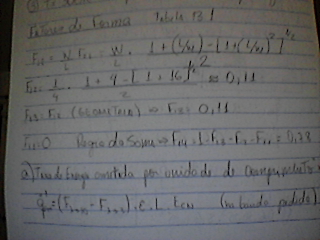
\includegraphics[scale=0.48]{./fig/3.png}
% \caption{\label{fig:tur}Grafico T x X } 
% \end{center}
% \end{figure}

% \myfig[scale=.48]{figPME2360-20111017-03}{Grafico $T \times X$}

Temperatura superficial uniforme:
\[ \frac{dT_{m}}{dx} = \frac{hP(T_{S}-T_{m})}{\dot{m}c}\]

\[\theta=T_{S}-T_{m} \]

Logo $d \theta = -dT_{m}$

\[\frac{d\theta}{dx}=-\frac{hP}{\dot{m}c}\theta\]

\[\ln (\theta)|_{\theta_{e}}^{\theta}= - \frac{hPx}{\dot{m}c}\]

\[\frac{\theta}{\theta_{e}}= \exp (- \frac{hPx}{\dot{m}c})\]

\[\frac{T_{m}-T_{s}}{T_{m,e}-T_{s}}= \exp (- \frac{hPx}{\dot{m}c})\]

\subparagraph*{8.4 Escoamento laminar em tubos circulares}

\paragraph*{reg desenvolvida}

Para $q''_{S}\ cte$: 
\[N_{Ud}=4.36\]
Para $T_{S}\ cte$: 
\[N_{Ud}=3.66\]

\paragraph*{reg. de entrada}

$T_{S}\ cte$

\[\bar{N}_{UD}=3.66+\frac{0.668(D/L)Re_{D}P_{r}}{1+0.04[((D/L)Re_{D}Pr)]^{\frac{2}{3}}}\]

Onde $[((D/L)Re_{D}Pr)]$ é o numero de Graetz ($Gz_{D}$) e com 
\[\bar{N}_{UD}=\frac{\bar{hD}}{k} \]

Válida para comprimento de entrada e comprimento de entrada combinada se $Pr >=5$

\subparagraph*{Seidel e Tate (comp. de entrada comb.)}

\[\bar{N}_{UD}=1.86( \frac{Re_{D}Pr}{L/D} )( \frac{\mu}{\mu_{S}} )\]

com $N_{Ud}>3.66$

\[0.6 <= Pr <= 5\]

\[0.0044 <= \frac{\mu}{\mu_{S}} <= 9.75\]

\subsection*{8.5 Escoamento turbulento em tubos circulares}

Dittus-Boelter: 
\[N_{UD}=0.023Re_{D}^{\frac{4}{5}}(Pr)^{n}\]
Com n = 0.4, $Ts > Tm$ e $0.7 <=Pr<=100$
E para n = 0.3, $Ts < Tm$ e $Re_{D}>=10000, L/D >=10$

\paragraph*{Bibliografia} Figuras retiradas de Incropera - Fundamentals of Heat and Mass Transfer-Incropera (6\textordfeminine edicao)

%pme2360
\section{Ex. 8.63}

% \begin{figure}[h]
% \begin{center}
% 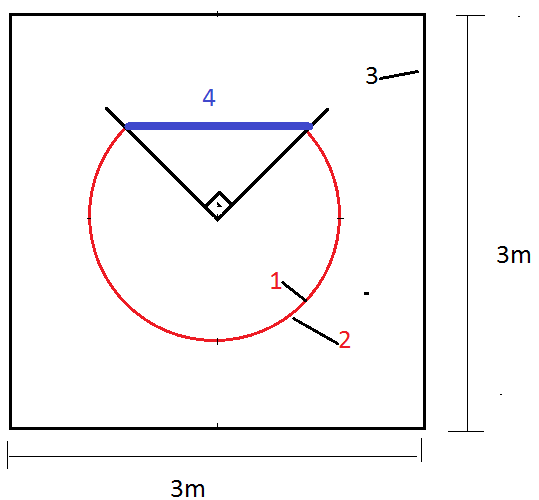
\includegraphics[scale=0.48]{./fig/1.png}
% \caption{\label{fig:1}fig 1} 
% \end{center}
% \end{figure}

\myfig[scale=.48]{figPME2360-20111019-01}{}

\begin{itemize}
\item $\rho$=900kg/m$^{3}$
\item $c_{0}$=200J/kgK
\item $\upsilon_{0}$=8.5*10$^{-4}$m$^{2}$/s
\item $k_{0}$=0.140 W/mK
\item $P_{R0}$=10$^{4}$ 
\end{itemize}

\paragraph*{Solução}

\[R_{eq}=\frac{1}{\bar{h} Pdx}+\frac{\ln(\frac{D_{0}}{D_{i}})}{2\pi dx k_{I}} \footnote{resistencia a conducao para uma parede cilindrica}+\frac{1}{sk_{s}}\]
s(tabela 4.1)-cilindro horizontal isotérmico de comprimento L enterrado em um meio semi-infinito

Para L $>>$ D
\[s'=\frac{2\pi L}{arccosh(\frac{2z}{D_{0}})}\]
\[s=s'\frac{dx}{L}\]
\[R_{eq}=\frac{1}{\bar{h} Pdx}+\frac{\ln(\frac{D_{0}}{D_{i}})}{2\pi dx k_{I}}+\frac{arccosh(\frac{2z}{D_{0}})}{2\pi dx k_{S}}\]

\[R_{eq}=\frac{R_{eq}'}{dx}\]
Balanço de energia

% \begin{figure}[h]
% \begin{center}
% 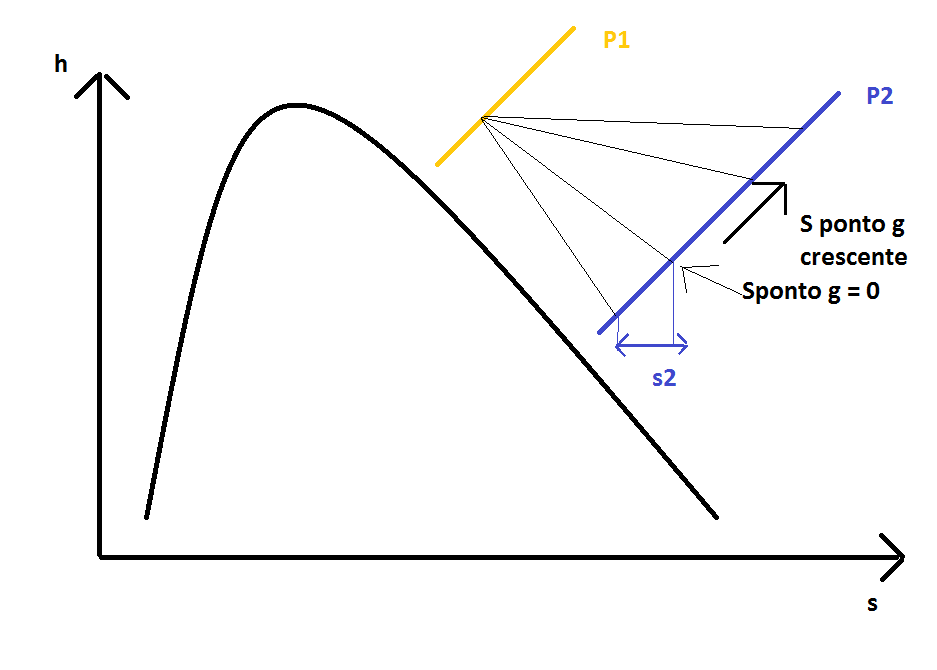
\includegraphics[scale=0.48]{./fig/2.png}
% \caption{\label{fig:1}fig 2} 
% \end{center}
% \end{figure}

\myfig[scale=.48]{figPME2360-20111019-02}{}

\[\dot{m}c_{0}T_{m}-\dot{m}c_{0}(T_{m}+dT_{m})+q''Pdx=0\]
\[\dot{m}c_{0}dT_{m}=q''Pdx\]
com:
\[q=\frac{Ts-Tm}{R_{eq}}\]
\[q''=\frac{Ts-Tm}{PdxR_{eq}}\]
\[\dot{m}cdT_{m}=\frac{T_{s}-T_{m}}{R'_{eq}}dx\]
\[dT_{m}=\frac{(T_{s}-T_{m})}{\dot{m}c_{0}R'_{eq}}dx\]

\[\theta = T_{s}-T_{m}\]
Portanto:
\[d\theta = -dT_{m}\]

\[d\theta = -\frac{\theta}{\dot{m}c_{0}R'_{eq}}dx\]

\[\int_{\theta _{e}}^{\theta _{s}}{\frac{d\theta}{\theta}}=\int_{x=0}^{x=L}{-\frac{dx}{\dot{m}c_{0}R'_{eq}}}\]

\begin{equation}
\frac{T_{m,s}-T_{s}}{T_{m,e}-T_{s}}=\exp(-\frac{L}{\dot{m}c_{0}R'_{eq}})
\label{eq:1}
\end{equation}


Cálculo de $\bar{h} $
\[
Re_{D}=\frac{\bar{\mu D_{i}}}{\upsilon _{0}}=\frac{\dot{m} D_{i}}{\upsilon _{0}\rho _{0} A_{tr}}\]
Onde $A_{tr}$=$\frac{\pi D_{i}^{2}}{4}$
\[\dot{m}=\rho _{0} \bar{\mu } A_{tr}\]
\[Re_{D}=\frac{4\dot{m}}{\upsilon _{0} \rho _{0} \pi D_{i}}=\frac{4*500}{8,5*10^{-4}*900*\pi * 1.2}=694\]

Como o resultado $<$ 2300, o regime é laminar

\[x_{CD,\upsilon}=0.05Re_{D}D\]
\[x_{CD,t}=x_{CD,\upsilon}*Pr\]

\[x_{CD,t}=4.16*10^{5}m\]

Estamos na região de entrada. Hausen $T_{sup}$ cte - interior do tubo.
\[\bar{Nu}_{D}=3.66+\frac{0.0668(\frac{D_{i}Re_{D}P_{R}}{L})}{1+0.04[\frac{D_{i}}{L}Re_{D}P_{R}]}=6.82\]

\[P_{r}>5\]
\[\bar{h}=\frac{Nu_{D}D_{I}}{k_{0}}=0.8W/m^{2}K\]

\[R_{eq}=\frac{1}{\bar{h} P}+\frac{\ln(\frac{D_{0}}{D_{i}})}{2\pi  k_{I}}+\frac{arccosh(\frac{2z}{D_{0}})}{2\pi  k_{S}}\]

\[R'_{eq}=0.33+0.71+0.66=1.7Km/W\]

\[\dot{q}=\dot{m}c_{0}(T_{m,e}-T_{m,s})=9.1*10^{6}W\]
Da equaçao \ref{eq:1}  $T_{m,s}$=111ºC

\section{8.60}  62 da 5a ed.

% \begin{figure}[h]
% \begin{center}
% 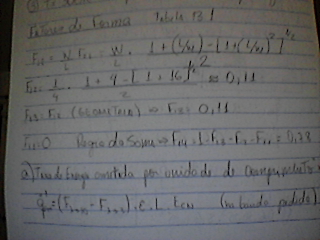
\includegraphics[scale=0.48]{./fig/3.png}
% \caption{\label{fig:1}fig 3} 
% \end{center}
% \end{figure}

\myfig[scale=.48]{figPME2360-20111019-03}{}

\begin{verbatim}
Entregar no dia da P2.
Tubo de parede delgada é usado pra transportar gases.
gas entra no tubo... ventos a uma temp de 15ºC em direcao
cruzada ao tubo a 5m/s. Considere as propriedades termofisicas
Estime coeficientes...

Temp media do fluido na saida -> balanço de volume de controle 
infinitesimal. Igual ao inicio do exercicio anterior. 
Temos 2 fluidos trocando energia entre quantas
resistencias em série? R: 3 (a de conveccao, a de conducao 
(parede do tubo) e a de conveeccao )
\end{verbatim}

\[R_{eq}=\frac{1}{h_{i}A_{i}} + cond\footnote{praticamente 0} + \frac{1}{h_{e}A_{e}}\]
Precisa verificar qual tipo de escoamento: no caso é turbulento.
Precisa verificar qual as regiões de entrada: 10 x o diametro. Tem 60 mm de comprimento.
A correlaçao que a gente usa é a Dittus- (Reynolds + Prandt)
Cálculo de $h_{i}$Eu avalio em qual temperatura? R: T média entre a entrada e a saída.
Deverá imaginar e chutar uma temperatura na saída. Avaliar as temperaturas médias e verificar o que resulta.

Cálculo de $h_{e}$:Kukauskas

\[Nu_{D}=cRe^{m}(\frac{Pr}{Pr_{S}})^{\frac{1}{4}}Pr^{n}\]

\[P_{R} \ de\  T _{\infty} \]

\[h_{i}(T_{m}-T_{s})=h_{e}(T_{S}-T_{\infty})\]

%pme2360
\section{Convecção Natural x Conveccção Forçada}
É muito semelhante ao que nós ja fizemos para convecção forçada.\\
Agente externo provocando o movimento do fluido: convecção forçada.
O que define convecção natural: transferência de calor devido a diferença
de temperatura.
Convecçao Mista: mistura das outras duas anteriores.
É possível calcular um numero de Nusselt que seja a soma das conveccoes 
natural e forçada.

% \begin{figure}[h]
% \begin{center}
% 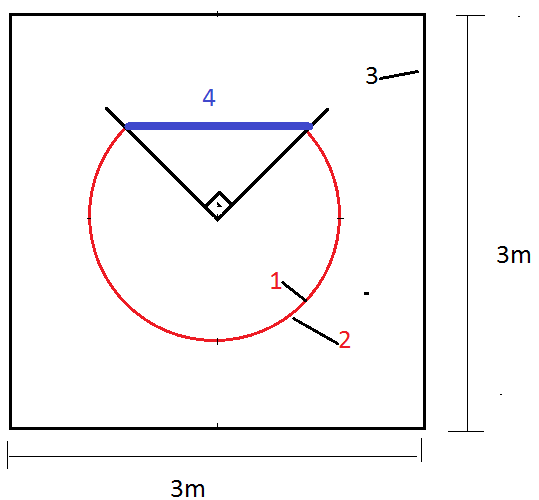
\includegraphics[scale=0.18]{./fig/1.png}
% \caption{\label{fig:1}1} 
% \end{center}
% \end{figure}

% \myfig[scale=.18]{figPME2360-20111026-01}{}

Se eu tenho um fluido quente embaixo e um fluido frio em cima formam-se correntes de convecção.

Em conveccçao forçada, os coeficientes nao dependiam da temperatura.
Agora, em convecção mista, também vão depender.

% \begin{figure}[h]
% \begin{center}
% 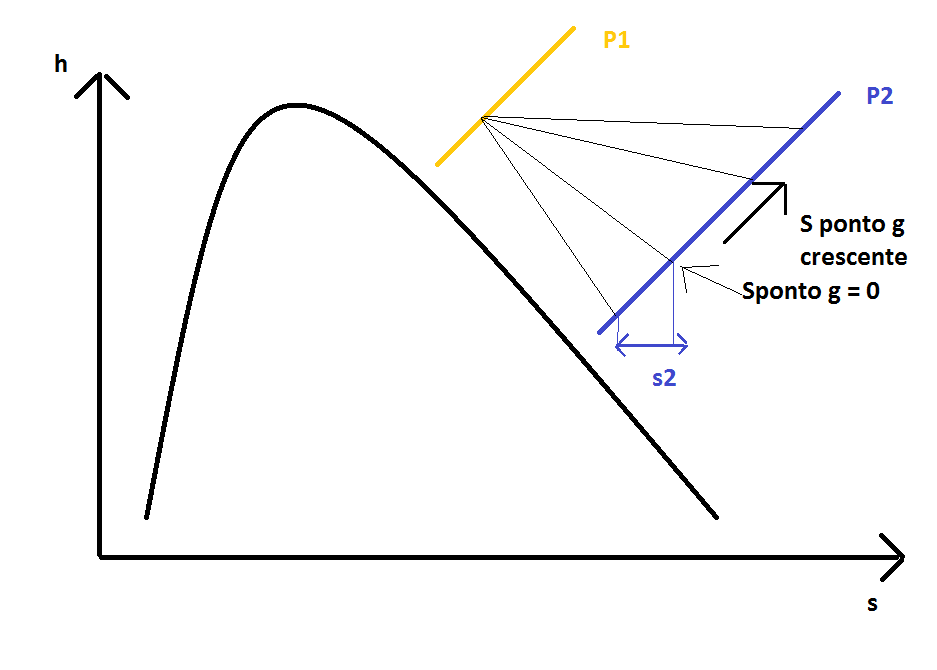
\includegraphics[scale=0.18]{./fig/2.png}
% \caption{\label{fig:2}2} 
% \end{center}
% \end{figure}

% \myfig[scale=.18]{figPME2360-20111026-02}{}

Quantidade de movimento na direçao x:
\begin{equation}
u\frac{du}{dx}+v\frac{du}{dy}=-\frac{1}{\rho}\frac{dp_{\infty}}{dx}-g+v\frac{d^{2}u}{dy^{2}}
\label{eq:1}
\end{equation}

Fora da camada limite:
\begin{equation}
\frac{dp_{\infty}}{dx}=-\rho_{\infty}g
\label{eq:2}
\end{equation}
\[\Delta \rho = \rho _{\infty}-\rho\]
Combinando as equações \ref{eq:1} e \ref{eq:2}
\begin{equation}
u\frac{du}{dx}+v\frac{du}{dy}=g\frac{\Delta \rho}{\rho}+v\frac{d^{2}u}{dy^{2}}
\label{eq:3}
\end{equation}

% \begin{figure}[h]
% \begin{center}
% 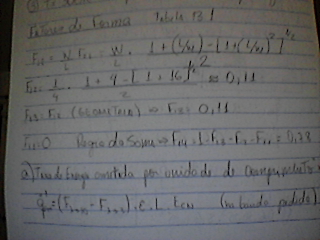
\includegraphics[scale=0.18]{./fig/3.png}
% \caption{\label{fig:3}3} 
% \end{center}
% \end{figure}

% \myfig[scale=.18]{figPME2360-20111026-03}{}

Coeficiente de expansão volumétrica:
\begin{equation}
\beta=-\frac{1}{\rho}(\frac{d\rho}{dt})=\footnote{aproximacao de Boussinesq} -\frac{1}{\rho}\frac{\rho _{\infty}-\rho}{T_{\infty}-T}
\end{equation}

\begin{equation}
\rho _{\infty}-\rho=-\rho\beta(T_{\infty}-T)
\label{eq:4}
\end{equation}

Combinando as equações \ref{eq:3} e \ref{eq:4}
\begin{equation}
u\frac{du}{dx}+v\frac{du}{dy}=g\frac{\beta (t_{S}-T_{\infty})}{u_{0}^{2}}T+\frac{1}{Re_{L}}\frac{d^{2}u}{dy^{2}}
\end{equation}

\newpage

\[u^{*}\frac{du^{*}}{dx^{*}}+v^{*}\frac{du^{*}}{dy^{*}}=g\frac{\beta (t_{S}-T_{\infty})}{u_{0}^{2}}T^{*}+\frac{1}{Re_{L}}\frac{d^{2}u^{*}}{dy^{*2}}
\]


\[u^{*}\frac{dT^{*}}{dx^{*}}+v^{*}\frac{dT^{*}}{dy^{*}}= \frac{1}{Re_{L}Pr}\frac{d^{2}T}{dy^{*2}}\]

\[u^{*}\frac{du^{*}}{dx^{*}}+v^{*}\frac{du^{*}}{dy^{*}}=\frac{Gr_{L}}{Re_{L}^{2}}T^{*}+\frac{1}{Re_{L}}\frac{d^{2}u^{*}}{dy^{*2}}
\]

\[u^{*}\frac{dT^{*}}{dx^{*}}+v^{*}\frac{dT^{*}}{dy^{*}}= \frac{1}{Re_{L}Pr}\frac{d^{2}T}{dy^{*2}}\]

Espera-se 
\[Nu_{L}=f(Re_{L},Gr_{L},Pr)\]

Condições de contorno:
\begin{itemize}
\item y = 0, u = v = 0, T=$T_{S}$
\item y$ \rightarrow \infty$, u $\rightarrow$0, T$\rightarrow T_{\infty}$
\end{itemize}

O que acontece quando você varia a espessura da camada limite? A variaçao da velocidade é menor com a maior espessura da camada limite (devido ao numero de Nusselt).

Parametro de similaridade:
\[\eta=\frac{y}{x}(\frac{Gr_{x}}{4})^{\frac{1}{3}} \]

\[f'''+3ff''-2(f')^{2}+T^{*}=0\]

\paragraph*{Exemplo} 
placa vertical com $T_{S}$ uniforme de 130º C e ar quiescente a 25º C. Determinar $\delta$ e $u_{max}$ para x=0.25 m

\[T_{f}=350K\]
\[Pr=0.7\]
\[Gr_{x}=6.718*10^{9}x^{3}\]
\[\nu = 20.92*10^{6}m^{2}/s\]
\[\eta = \frac{y}{x}(\frac{Gr_{x}}{4})^{1/4}=\frac{\delta}{0.25}(\frac{6.718*10^{9}*0.25^{3}}{4})^{1/4}=5\]

\[\delta = 1.746*10^{-3}m=17.5mm\]

\[u_{max}=0.47m/s\]
\[f'(n)=\frac{ux}{2\upsilon}Gr_{x}^{-1/2}=0.275\]

% \begin{figure}[h]
% \begin{center}
% 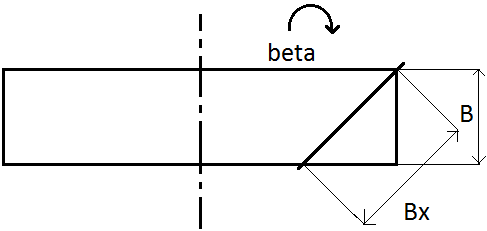
\includegraphics[scale=0.38]{./fig/4.png}
% \caption{\label{fig:4}4} 
% \end{center}
% \end{figure}

% \myfig[scale=.18]{figPME2360-20111026-04}{}

\[Nu_{x}=(\frac{Gr_{x}}{4})g(Pr)=(\frac{6.718*10^{9}*0.25^{3}}{4})*0.5=35.8\]
\[h=35.8*0.030/0.25=4.3W/m^{2}K\]
\[g(Pr)=\frac{0.75Pr^{1/2}}{(0.609+1.22Pr^{1/2})}\]

\[Ra_{x,c}=Gr_{x,c}Pr=6.718*10^{9}x^{3}*0.7\]

%pme2360
\section{12.44}

% \begin{figure}[h]
% \begin{center}
% 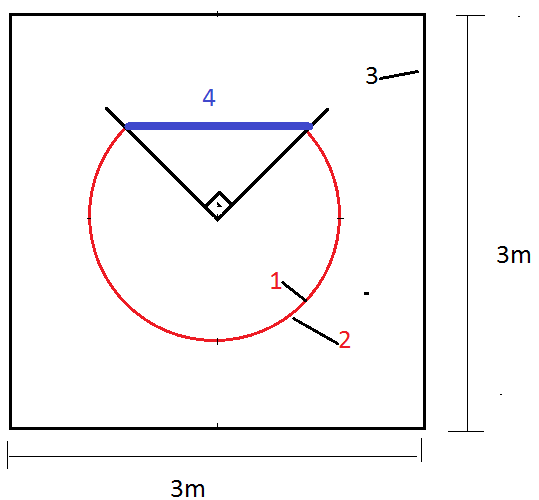
\includegraphics[scale=0.28]{./fig/1.png}
% \caption{\label{fig:1}1} 
% \end{center}
% \end{figure}

\myfig[scale=.28]{figPME2360-20111116-01}{}

\subsection{a) emissividade total e absorvidade total}

Quer que calculemos $\varepsilon$ (poder emissivo espectral de um corpo negro) e $\alpha$


\begin{verbatim}
Emissividade total computa a radiação emitida por toda uma superfície
poder emissivo espectral de um corpo negro
emissividade também depende da temperatura da superfície
3 niveis da lei de kirchhoff
\end{verbatim}

\[\varepsilon = \frac{\int _{0} ^{\infty} {\varepsilon(\lambda)E_{CN,\lambda(\lambda ,T)}}d\lambda}{E_{CN}(T)}\]

\[\alpha = \frac{\int _{0}^{\infty}\alpha _{\lambda}G(\lambda)d\lambda }{G}\]

\[
\varepsilon = \frac{\int _{0}^{1\mu m}\varepsilon _{\lambda}E_{CN,\lambda}}{E_{CN}(T)} + \frac{\int _{1}^{3\mu m}\varepsilon _{\lambda}E_{CN,\lambda}}{E_{CN}(T)} + \frac{\int _{3}^{1\infty}\varepsilon _{\lambda}E_{CN,\lambda}}{E_{CN}(T)}
\]

\[
\varepsilon = \varepsilon _{1 \rightarrow 3} \frac{\int _{0}^{1\mu m}\varepsilon _{\lambda}E_{CN,\lambda}}{E_{CN}(T)} +  \varepsilon _{3 \rightarrow \infty} \frac{\int _{1}^{3\mu m}\varepsilon _{\lambda}E_{CN,\lambda}}{E_{CN}(T)} 
\]

\[
\varepsilon = \varepsilon _{1 \rightarrow 3} \times F_{1 \rightarrow 3\mu m} +  \varepsilon _{3 \rightarrow \infty} \times F_{3 \rightarrow  \infty}
\]

Em que

\begin{itemize}
\item $ F_{1 \rightarrow 3\mu m}$ = $F_{0 \rightarrow 3} - F_{0 \rightarrow 1}$
\item $ F_{3 \rightarrow \infty}$ = $1 - F_{0 \rightarrow 3}$
\end{itemize}


Consultar a tabela 12.1

\[
\lambda T = 1 \mu m \times 400K = 400 \mu mK \rightarrow F_{0 \rightarrow 1\mu m} = 0.000000
\]

\[
\lambda T = 3 \mu m \times 400K = 1200 \mu mK \rightarrow F_{0 \rightarrow 3\mu m} = 0.002134
\]

\[
\varepsilon = 0.7 \times (0.002134 - 0.000000)+0.5 \times (1-0.002134)
\]

\[\varepsilon = 0.500\]

% \begin{figure}[h]
% \begin{center}
% 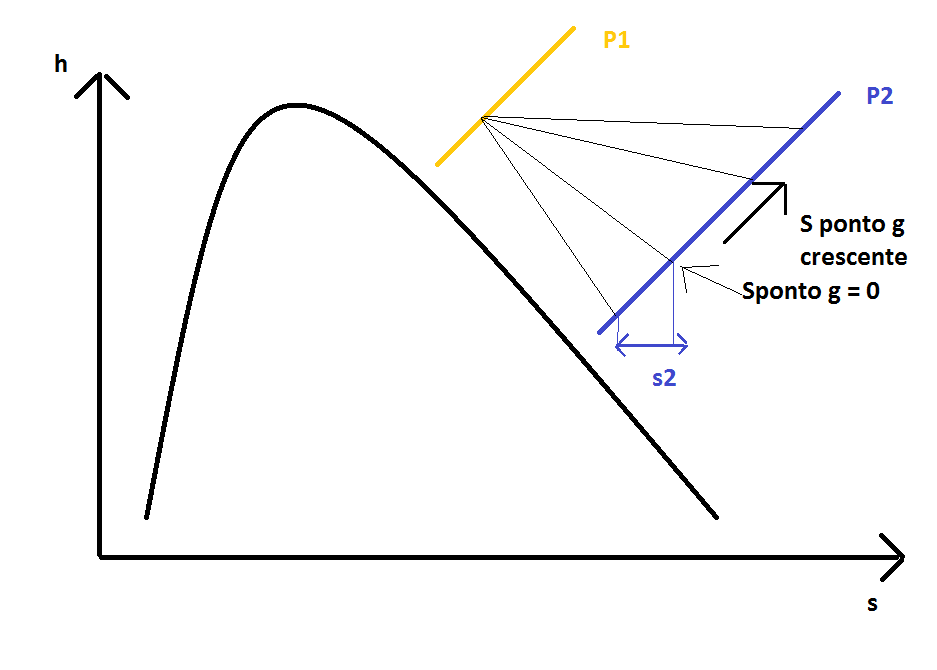
\includegraphics[scale=0.28]{./fig/2.png}
% \caption{\label{fig:2}2} 
% \end{center}
% \end{figure}

\myfig[scale=.28]{figPME2360-20111116-02}{}

Difusa:

\begin{itemize}
\item $\varepsilon _{\lambda} = \alpha _{\lambda}$
\item $G(\lambda) = E_{CN,\lambda}(T_{f})$
\end{itemize}

Em que $E_{CN,\lambda}$ é a do forno.
\[G = E_{CN}(T_{f})\]

\[
\alpha = \alpha _{1 \rightarrow 3}F_{1 \rightarrow 3} + \alpha _{3 \rightarrow \infty}F_{3 \rightarrow \infty}
\]

\[
\lambda T = 1 \mu m \times 2000K = 2000 \mu mK \rightarrow F_{0 \rightarrow 1\mu m} = 0.066728
\]

\[
\lambda T = 3 \mu m \times 2000K = 6000 \mu mK \rightarrow F_{0 \rightarrow 3\mu m} = 0.737818
\]

\[
\alpha = 0.7 \times (0.737818 - 0.066728)+0.5 \times (1-0.0.737818)
\]

\[\alpha = 0.6\]


\subsection{b) refletida}

\[(1-\alpha)G=0.4 \times \sigma \times 2000^{4} = 3.621 \times 10 ^{5} W/m^{2}\]
Líquido:

\[q'' = \alpha G - \varepsilon E_{CN}(T_{s})\]
Em 	que G = $E_{CN}(T_{f})$

\[q'' = \alpha \sigma T_{f}^{4} - \varepsilon  \sigma T_{s}^{4}\]
\[q'' = 5.45 \times 10^{5} W/m^{2}\]

\subsection{c)$E_{\lambda=2 \mu m}(T_{s}) = ?$  }


\[E_{\lambda , CN}\]

\[
E_{\alpha} = 2 \mu m = \varepsilon _{\lambda} = 2 \mu E_{CN,\lambda}
\]

Consultar a tabela 12.1:\ \ \ \ \ 
\begin{tabular}{|c|c|}
\hline 
$\lambda T$ & $\frac{I_{\lambda , CN}}{\sigma T^{5}}$ \\ 
\hline 
• & • \\ 
\hline 
\end{tabular} 

\[E_{CN,\lambda} = \pi I_{\lambda,CN}\]
Em que a unidade de $E_{CN,\lambda}$ é $W/(m^{2} \mu m)$

Para $\lambda T = 2 \times 400 = 800 \mu mK$

\[
\frac{I_{\lambda , CN}}{\sigma T^{5}\footnote{400 K}} = 0.991126 \times 10^{-7}
\]

\[
I_{\lambda , CN} = 0.0575 \frac{W}{m^{2} \mu m }
\]

\[E_{\lambda=2 \mu m} = 0.7 \times \pi \times  0.0575 = 0.126 \frac{W}{\mu m m^{2}}\]

\subsection{d) $\lambda _{1/2} = ?$}

Para$ F_{0 \rightarrow \lambda 1/2} = 0.5$.
Da tabela,

\[
\lambda T = 4100 \mu m K
\]
Onde T = 400 K
\[\lambda _{1/2} = 10.3 \mu m\]

\pagebreak

\section{13.119}

% \begin{figure}[h]
% \begin{center}
% 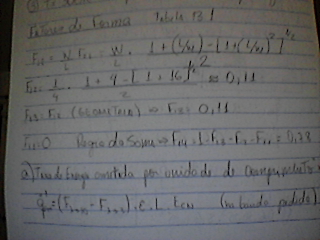
\includegraphics[scale=0.28]{./fig/3.png}
% \caption{\label{fig:3}3} 
% \end{center}
% \end{figure}

\myfig[scale=.28]{figPME2360-20111116-03}{}

% \begin{figure}[ht]
% \subfigure[4]{
% \label{fig:4}
% 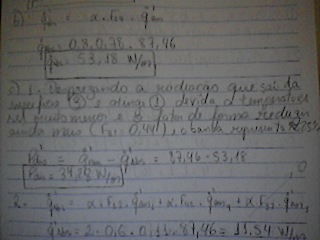
\includegraphics[scale=0.26]{./fig/5.png}
% }
% \subfigure[5]{
% \label{fig:5}
% 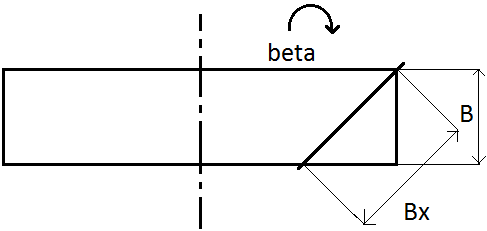
\includegraphics[scale=0.26]{./fig/4.png}
% }
% \caption{\label{fig:6}}
% \subref{fig:4} ,\subref{fig:5}
% \end{figure}

\myfig[scale=.28]{figPME2360-20111116-05}{}

\myfig[scale=.28]{figPME2360-20111116-04}{}

\[\frac{1}{A_{1}} \left[  \frac{1-\varepsilon_{1}}{\varepsilon_{1}} + \frac{1}{F_{12}=1  } + \frac{1-\varepsilon _{2}}{\varepsilon _{2} A_{2}/A_{1}} \right]\]

\begin{verbatim}
Falta a energia que sai do circuito. 3 superfícies equivalem a 3 nós. 
Qual a superfície do 3º nó?
\end{verbatim}

%pme2360-ex
\section{Fator de Forma}
O fator de forma $F_{ij}$ é definido como \textit{ a fração da radiação que deixa a superfície i que é interceptada pela superfície j}. Considerando as superfícies $A_{i}$ e $A_{j}$ orientadas arbitrariamente conforme a figura \ref{fig:2}

% \begin{figure}[h]
% \begin{center}
% 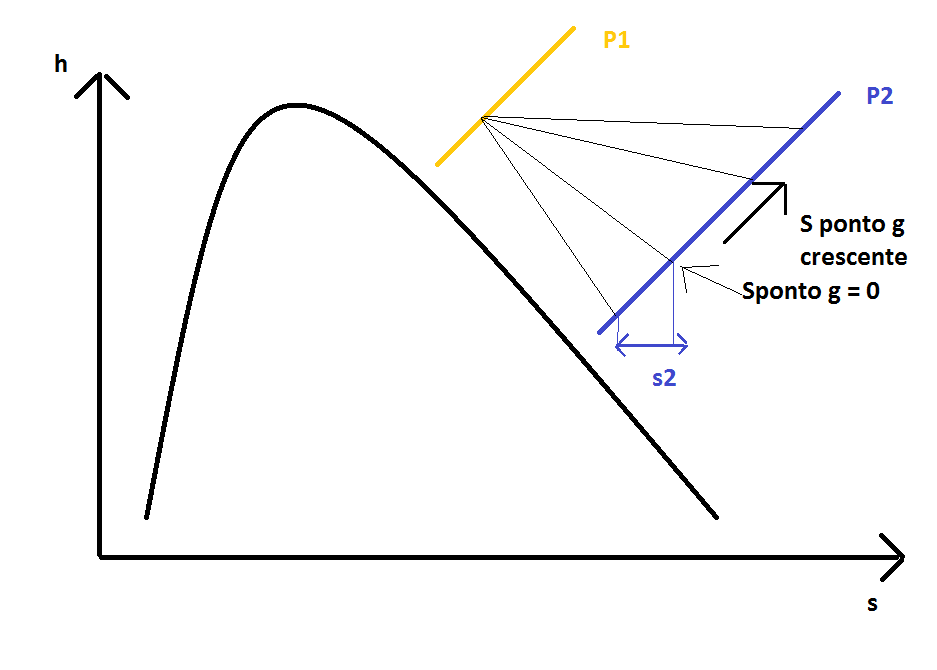
\includegraphics[scale=.35]{./fig/2.png}
% \caption{\label{fig:2}Fator de forma associado com a troca de radiação entre elementos de superfície de área $dA_{i}$ e $dA_{j}$}
% \end{center}
% \end{figure}

\myfig[scale=.35]{figPME2360-20111116-01e}{Fator de forma associado com a troca de radiação entre elementos de superfície de área $dA_{i}$ e $dA_{j}$}

Áreas elementares em cada superfície $dA_{i}$ e $dA_{j}$ são conectadas por uma reta de comprimento R, formando ângulos polares $\theta _{i}$ e $\theta _{j}$ com relação às normais $\textbf{n}_{i}$ e $\textbf{n}_{j}$. Os valores de R, $\theta _{i}$ e $\theta _{j}$ variam de acordo com as posições das áreas elementares $dA_{i}$ e $dA_{j}$.

A taxa na qual a radiaçao deixa $dA_{i}$ e é interceptada por $dA_{j}$ é definida como :

\[dq_{i \rightarrow j} = I_{i}\cos(\theta _{i})dA_{i}d\omega _{j-i}\]

Onde:
\begin{itemize}
\item $I_{i}$ é a intensidade da radiação que deixa a superfície $i$
\item $d\omega _{j-i}$ é o ângulo sólido subtendido por $dA_{j}$ visto de $dA_{i}$
\end{itemize}

Sendo $d\omega _{j-i}$ = ($\cos\theta_{i}\cos\theta_{j}$)/$R^{2}$, segue que:

\[dq_{i \rightarrow j} = I_{i}\frac{\cos\theta_{i}\cos\theta_{j}}{R^{2}}dA_{i}dA_{j} \]

Se a superfície \textit{i} emite e reflete difusamente ( $J = \pi I_{e+r}$), temos:

\[
	dq_{i \rightarrow j} = J_{i}\frac{\cos\theta_{i}\cos\theta_{j}}{\pi R^{2}}dA_{i}dA_{j} 
\]

A taxa total na qual a radiação deixa a superfície \textit{i} e é interceptada por \textit{j} é obtida, portanto, integrando-se sobre as duas superfícies:

\[
	q_{i \rightarrow j} = J_{i} \int _{A_{i}} \int _{A_{j}} \frac{\cos\theta_{i}\cos\theta_{j}}{\pi R^{2}}dA_{i}dA_{j} 
\] 

Onde $J_{i}$ é considerada uniforme sobre a superfície $A_{i}$.

Da definição de fator de forma como sendo a fração da radiaçao que deixa $A_{i}$ e chega em $A_{j}$:

\[F_{ij}=\frac{q_{i \rightarrow j}}{A_{i}J_{i}}\]

Temos que o fator de forma é definido por:

\[
	F_{ij} = \frac{1}{A_{i}} \int _{A_{i}} \int _{A_{j}} \frac{\cos\theta_{i}\cos\theta_{j}}{\pi R^{2}}dA_{i}dA_{j} 
\] 

\pagebreak

\section{Troca Radiante entre Superfícies}
Seja $q_{i}$ a taxa \textit{líquida} na qual a radiação deixa uma superfície $i$, representada por:

\begin{equation}
q_{i}=A_{i}(J_{i}-G_{i})
\label{eq:1}
\end{equation}

A irradiação da superfície $i$ pode ser calculada a partir das radiosidades de todas as superfícies no invólucro. Em particular, da definiçao de \textit{fator de forma}, a taxa total de radiação atingindo a superfície $i$ oriunda de todas as superfícies, incluindo $i$ é:

\[A_{i}G_{i}=\sum _{j=1}^{N}{F_{ji}A_{j}J_{j}}\]
Ou, usando a relação de reciprocidade, 

\begin{equation}
A_{i}G_{i}=\sum _{j=1}^{N}{A_{i}F_{ij}J_{j}}
\label{eq:2}
\end{equation}

Eliminando a área $A_{i}$ e substituindo \ref{eq:2} em \ref{eq:1}

\begin{equation}
q_{i}=A_{i}\left(  J_{i} - \sum _{j=1}^{N}{F_{ij}J_{j}}  \right)
\label{eq:3}
\end{equation}

Seja a relação da Regra do Somatório:

\begin{equation}
\sum _{j=1}^{N}{F_{ij}} = 1
\label{eq:4}
\end{equation}

De \ref{eq:4} em \ref{eq:3}:
\[
q_{i}=A_{i}\left(  \sum _{j=1}^{N}{F_{ij}}J_{i} - \sum _{j=1}^{N}{F_{ij}J_{j}}  \right)
\]
\\
Logo, usando a propriedade de linearidade da somatória

\begin{equation}
q_{i}=\sum _{j=1}^{N}{A_{i}F_{ij}(  J_{i} - J_{j}  )} = \sum _{j=1}^{N}q_{ij}
\label{eq:5}
\end{equation}

Ou seja, a taxa \textit{líquida} na qual a radiação deixa uma superfície $i$ equivale à soma das componentes $q_{ij}$ relativas à troca radiativa com outras superfícies. Fazendo uma analogia a um circuito elétrico com seus vários componentes (figura \ref{fig:1}), temos:

\begin{itemize}
\item ($J_{i}-J_{j}$) = potencial motriz
\item ($A_{i}F_{ij}$) = resistência espacial ou geométrica
\end{itemize}

% \begin{figure}[h]
% \begin{center}
% 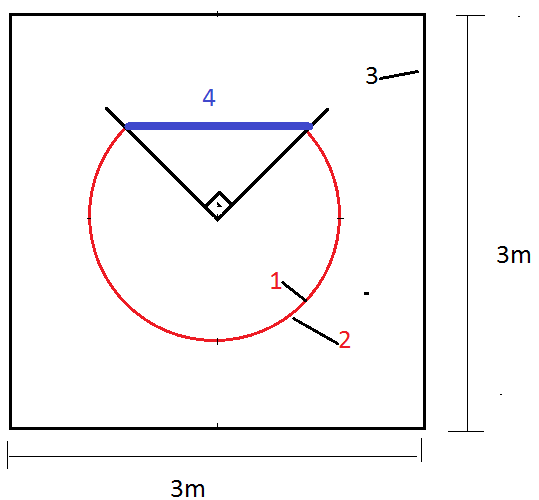
\includegraphics[scale=0.4]{./fig/1.png}
% \caption{\label{fig:1}representação do circuito equivalente}
% \end{center}
% \end{figure}

\myfig[scale=.4]{figPME2360-20111116-02e}{Representação do circuito equivalente}

Seja agora $q_{i}$ definida como:

\begin{equation}
q_{i}=\frac{E_{bi}-J_{i}}{(1-\varepsilon _{i})/\varepsilon _{i}A_{i}}
\label{eq:6}
\end{equation}

Em que $\varepsilon _{i}$ é a \textit{emissividade hemisférica total} da superfície $i$, $J_{i}$ é a \textit{radiosidade} da superfície, e $E_{b}$ o \textit{poder emissivo hemisférico total de um corpo negro}.

Combinando as equações \ref{eq:6} e \ref{eq:5}, temos:

\begin{equation}
\frac{E_{bi}-J_{i}}{(1-\varepsilon _{i})/ \varepsilon _{i}A_{i}} = \sum _{j=1}^{N} \frac{(  J_{i} - J_{j}  )} {(A_{i}F_{ij})^{-1}}
\label{eq:7}
\end{equation}

A equação \ref{eq:7} representa o balanço de radiação para o \textit{nó} da radiosidade associado com a superfície \textit{i} (figura \ref{fig:1}). E é especialmente útil quando a temperatura $T_{i}$ (e portanto $E_{bi}$) da superfície é conhecida.

\begin{equation}
q_{i} = \sum _{j=1}^{N} \frac{(  J_{i} - J_{j}  )} {(A_{i}F_{ij})^{-1}}
\label{eq:8}
\end{equation}

A equação \ref{eq:8} é especialmente importante quando a \textit{taxa de transferência líquida de radiação na superfície} é conhecida.

%pme2360
\section{Ex. 6}

% \begin{figure}[h]
% \begin{center}
% 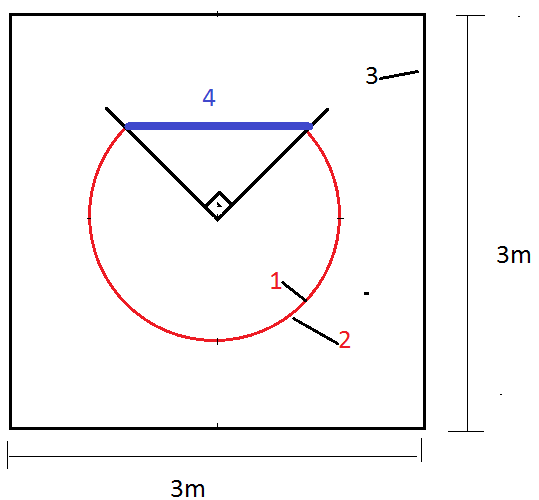
\includegraphics[scale=0.48]{./fig/1.png}
% \caption{\label{fig:1}1} 
% \end{center}
% \end{figure}

\myfig[scale=.48]{figPME2360-20111123-01}{}

\[T_{1} = T_{2} = 1000 \ K\]
\[T_{3} = 300 \ K\]
\[\varepsilon _{3} = \alpha _{3} = 0.2\]

\[\alpha _{3} = 0.2\]
\[\varepsilon _{1} = 0.3\]
\[\varepsilon _{2} = 0.5256\]
\[\alpha _{3} = 0.7180\]

% \begin{figure}[h]
% \begin{center}
% 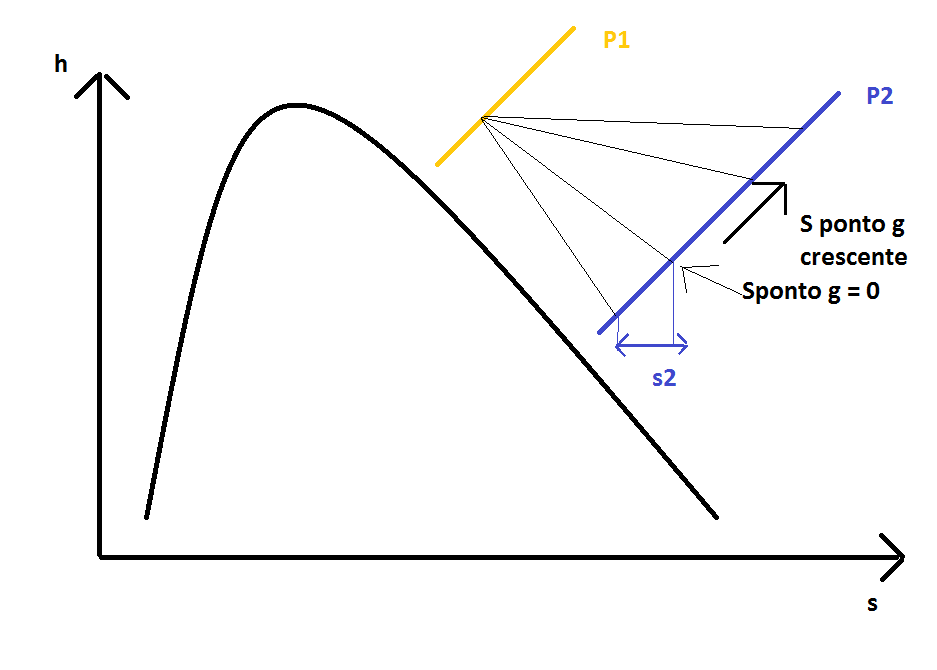
\includegraphics[scale=0.6]{./fig/2.png}
% \caption{\label{fig:2}2} 
% \end{center}
% \end{figure}

\myfig[scale=.48]{figPME2360-20111123-02}{}

\paragraph*{a} $\varepsilon _{2} = ? $
\paragraph*{b} $\alpha _{2} = ? $
\paragraph*{c} $q_{13} = ? $

\[R_{1} = \frac{1-\varepsilon _{1}}{\varepsilon _{1} A_{1}}\]
\[R_{2} = \frac{1-\varepsilon _{2}}{\varepsilon _{2} A_{2}}\]
\[R_{3} = \frac{1-\varepsilon _{3}}{\varepsilon _{3} A_{3}}\]

\[R_{13} = (A_{1}F_{13})^{-1}\]
\[R_{23} = (A_{2}F_{23})^{-1}\]


Superfície difusa: radiação não tem uma direção específica, a superfície emite em todas as direções.

Superfície Cinzenta: emissividade e absorvidade não dependem do comprimento de onda
O exercício tem que dizer que a superfície é cinzenta para podermos montar um circuito, tal como o usado na resolução.

Radiosidade é a contribuiçao líquida da radiação do corpo, e compreende o que o corpo emite e reflete menos o que ele absorve da radiação ambiente. O tipo de resistência que liga as radiosidades num circuito é a geométrica (que tem a ver com o fator de forma). As outras resistências são ditas superficiais, e medem a "distância" $\ $ da radiosidade da superfície do corpo em relação a um corpo negro.

A unidade de radiosidade é $W/m^{2}$. Se a superfície é cinzenta, $\varepsilon = \alpha$

% \begin{figure}[h]
% \begin{center}
% 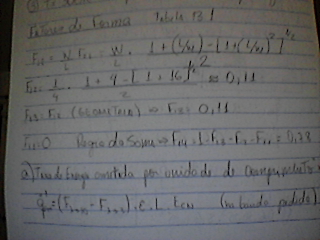
\includegraphics[scale=0.28]{./fig/3.png}
% \caption{\label{fig:3}Radiosidade} 
% \end{center}
% \end{figure}

\myfig[scale=.48]{figPME2360-20111123-03}{Radiosidade}

\[R_{1}' = \frac{1-0.3}{0.3 (2 \pi - \theta )R} = 0.4951 m^{-1}\]
Em que R vale 1 metro
\[R_{2}' = \frac{1-0.5256}{0.5256 (2 \pi - \theta )R} = 0.1914 m^{-1}\]

\[R_{3}' = \frac{1-0.2}{0.2 (2 \pi - \theta )R} = 0.333 m^{-1}\]

\[R_{13} = (0.3 (2 \pi - \theta )R)^{-1} = 0.707 m^{-1}\]
\[R_{23} = (1 (2 \pi - \theta )R)^{-1} = 0.2122 m^{-1} \]

\subsubsection{Cálculo dos Fatores de Forma}
A gente traça uma superfície fictícia, \textit{(4)}, e toda radiaçao que deixa \textit{(1)} e atinge \textit{(4)} também atinge \textit{(3)} (se \textit{(4)} não existisse).
O fator de forma $F_{41}$ = 1 (toda radiaçao que deixa \textit{(4)} (lado de dentro) atinge \textit{(1)})
Logo pela relação de reciprocidade,  
\[A_{4}F_{41} = A_{1}F_{14}\]
Portanto:
\[F_{14} = F_{13} = \frac{A_{4}}{A_{1}} F_{41}\]
Em que $F_{41}$ vale 1. 
\[F_{13} = \frac{2R\sin(\pi / 4) }{(2 \pi - \theta )R}\]
Em que $\theta$ vale $\pi /2$
 
$F_{23}$ = 1  (toda a radiação que deixa \textit{(2)} atinge \textit{(3)} $\rightarrow$ \textit{(2)} não pode atingir ela mesma)

\subsubsection{Soluçao do circuito}


\begin{itemize}
\item $q_{13}$ é a corrente que sai de $E_{CN,1}$ e chega em $J_{3}$
\item $q_{23}$ é a corrente que sai de $E_{CN,2}$ e chega em $J_{3}$
\item $q_{3}$ é a corrente que sai de $J_{3}$ e chega em $E_{CN,3}$
\end{itemize}

\[q_{13}' = \frac{E_{CN,1}-J_{3}}{R_{1}'+R_{13}'} = 0.8318(56690-J_{3})\]
Com $E_{CN,1}$ = $\sigma T_{1}^{4}$

\[q_{23}' = \frac{E_{CN,2}-J_{3}}{R_{2}'+R_{23}'} = 2.480(56690-J_{3})\]

\[q_{3}' = \frac{-E_{CN,3}+J_{3}}{R_{3}'} = 3.003(-459.19+J_{3})\]
Em que $E_{CN,3}$ = $\sigma T_{3}^{4}$

\[q_{3}'=q_{13}'+q_{23}'\]

\[J_{3} = 29949 \ W/m^{2}\]
\[q_{3}' = 88559 \ W/m (d)\]
\[q_{23}' = 66317 \ W/m \]
\[q_{13}' = 22243 \ W/m (c)\]

\subsection{E)}
$T_{2} = T_{1} = ? $ para $q_{3}$`= $2\times q_{3}'$ (item d) = $2 \times 88559$ = $177118 \ W/m$

\[\varepsilon _{2} = 0.2F_{0 \rightarrow 1} + 0.5(F_{0 \rightarrow 10}-F_{0 \rightarrow 1}) 0.8(1-F_{0 \rightarrow 10})\] 

Para T = 1000 K
\begin{itemize}
\item $F_{0 \rightarrow 10}$ = 0.914199
\item $F_{0 \rightarrow 1}$ = 0.000321
\end{itemize}

Para a nova temperatura, $F_{0 \rightarrow 10}$ (novo) $>$ $F_{0 \rightarrow 10}$ 
Hipótese: $F_{0 \rightarrow 10}$ (novo) = 1, portanto $\varepsilon _{2}^{(1)}$ = 0.5.

$F_{0 \rightarrow 1}$ = 0

\[177118 = 3.003(J_{3}-459.19)\]
\[q_{23}'=2.3562(E_{CN,1}-59439)\]
Em que $E_{CN,2}$ = $\sigma T_{1}^{4}$
\[q_{13}'=0.8318(E_{CN,1}-59439)\]

\[T_{1}^{1}=1193K\]


\[F_{0 \rightarrow 10} = 0.944378\]
\[F_{0 \rightarrow 1} = 0.002070\]

\[\varepsilon _{2}^{2} = 0.5173\]
\[T_{1}^{(2)}=1190 \ K\]

\[\varepsilon _{2}^{3} = \varepsilon _{2}^{2}\]

A gente duplicou a potência mas não sabemos qual a nova temperatura. Então, para resolver o item \textbf{e)}, só trocamos os potenciais e algumas resistências do circuito anterior. Nenhuma resistência geométrica mudou, apenas a da emissividade 2. Então o formato do circuito anterior continua válido, só que agora com as trocas dos valores de potenciais e resistências. 

Não sabemos os poderes emissivos dos corpos negros, mas sabemos $q_{13}$. Os potenciais são diferentes, e agora tenho que estimar os valores de emissividade. Temos que chutar uma emissividade. Achamos os valores de temperatura, achamos os valores de fração em cada banda, e então achamos a emissividade, e conferimos se bate com a emissividade chutada inicialmente.

\section{Trocadores de calor}
Calculos de trocador de calor, serve para (dado um trocador de calor), calcular as temperaturas na saída do trocador de calor, ou, dada uma temperatura final, determinar as dimensões desse trocador de calor.

O papel das chicanas é aumentar a superfície no interior do casco.

Trocadores de calor compactos tem áreas extremamente elevadas para volumes pequenos.
O fluido passa por passagens extremamente extensas e finas, com escoamento laminar.

%pme2360
\section{Exercício}

% \begin{figure}[h]
% \begin{center}
% 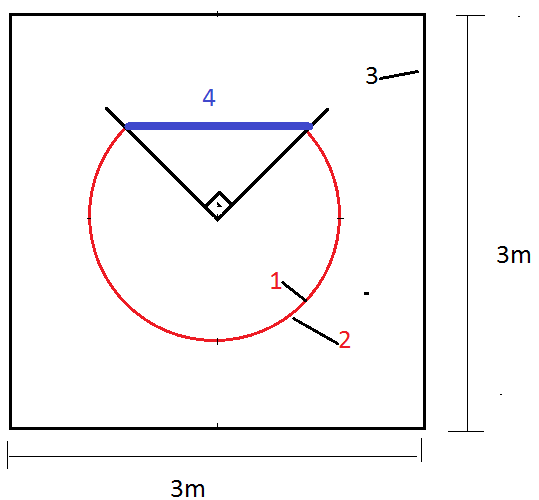
\includegraphics[scale=0.28]{./fig/1.png}
% \caption{\label{fig:1}1} 
% \end{center}
% \end{figure}

\myfig[scale=.28]{figPME2360-20111130-01}{}

\[\dot{m}_{oleo}=2Kg/s\]
\[T_{h,i} = 120ºC\]
\[T_{h,o} = 40ºC\]
\[c_{p,oleo} = 2118.0 J/kg\]

\[U = 3000 W/m^{2}K\]
\[T_{c,i} = 15ºC\]
\[T_{c,o}= 45ºC\]
\[c_{p,agua} = 4178 J/kg\]

\subsection{a}
\textit{vazão mássica de água}
\[\dot{m}_{oleo} \times c_{p,oleo} (T_{h,i}-T_{h,o}) = \dot{m} \times c_{p,agua}(T_{c,o}-T_{c,i})\]
\[2 \times 2118 \times (120-40) = \dot{m} * 4178 * ( 45-15 ) = \dot{q}=33880J/kg\]
\[\dot{m}_{agua}=2.70 \ kg/s\]

\subsection{b}
Trocador de casco-tubo

1 passe na carcaça

6 passes nos tubos

% \begin{figure}[h]
% \begin{center}
% 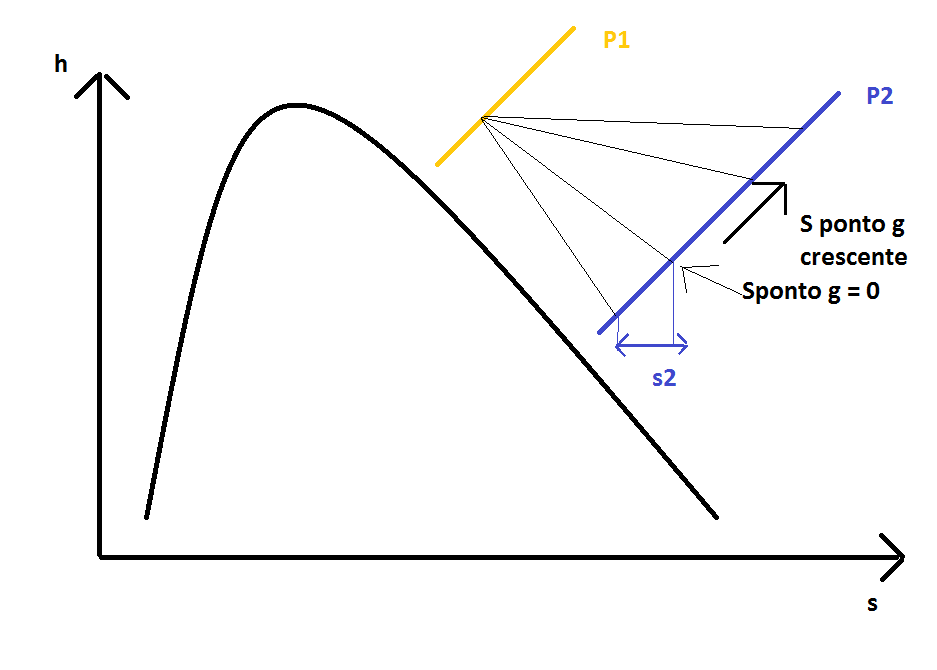
\includegraphics[scale=0.28]{./fig/2.png}
% \caption{\label{fig:2}Trocador em contra-corrente} 
% \end{center}
% \end{figure}

\myfig[scale=.28]{figPME2360-20111130-02}{}

\paragraph{Método MLDT}
Método Logarítmo para trocador de calor em corrente contrária

\[\Delta T_{lm,cc}=\frac{\Delta T_{1}-\Delta T_{2}}{\ln(\Delta T_{1}/\Delta T_{2})}\]
Em que lm é a média logarítmica e o cc é a corrente contrária

\[\Delta T_{1} = T_{h,i} - T_{c,o} = 120 - 45 = 75\]
\[\Delta T_{2} = T_{h,o} - T_{c,i} = 40 - 15 = 25\]

\[\Delta T_{lm,cc} = \frac{75-25}{\ln(75/25)}=45.5ºC\]

\[q = UA \Delta T_{lm,cc} F\]

Pela figura 11.10, (pag 459, 5a ed.)

\myfig[scale=.28]{figPME2360-20111130-03}{}

\[R = \frac{T_{e}-T_{s}}{t_{s}-t_{e}} = \frac{120-45}{45-15}=2.66\]
\[P = \frac{t_{s}-t_{e}}{T_{e}-t_{e}} = \frac{45-15}{120-15}=0.285\]

\[F = 0.85\]

\[338880=300 \times A \times 45,5 \times 0.85\]
\[A = 29.2 m^{2}\]

\subsection{c}
Do trocador:
\[A = N \pi D L \]

\[L = \frac{29.20}{25 \times 6 \times \pi \times 0.02} = 3.09 m\]

\section{Ex 11.35 da 6a Ed}

% \begin{figure}[h]
% \begin{center}
% 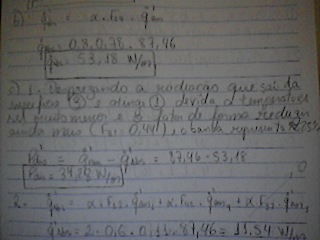
\includegraphics[scale=0.45]{./fig/5.png}
% \caption{\label{fig:3}3} 
% \end{center}
% \end{figure}

\myfig[scale=.28]{figPME2360-20111130-05}{}

Trocador de calor casco tubo

1 passe carcaça

2 passes no tubo

130 tubos de latão

\[\phi _{i} = 13.4mm\]
\[\phi _{e} = 15.9mm\]
\[2m/passe\]

- Escoamento Interno nos tubos

\[\bar{T}_{m}=\frac{20+40}{2}=30ºC\]

\[\rho = 997 kg/m^{3}\]
\[\mu = 855 \times 10^{-6}\]
\[c_{p} = 4179 J/kgK\]
\[Pr = 5.83\]
\[K = 613 \times 10^{-3}\]

\[Re = \frac{U \phi _{i}}{\nu} = \frac{U \phi _{i} \rho}{\mu}\]

\[Re = \frac{1.25 \times 0.0134 \times 997 } { 855 \times 10 ^{-6}} = 19531\]

Turbulento

L/D $>$ 10

\[\bar{Nu}_{D} = 0.023 Re_{D}^{4/5}Pr^{0.4}=126\]

\[\bar{h}=\frac{126 \times 613 \times 10^{-3}}{ 0.0134 } = 5767 W/m^{2}K\]

Coeficiente Global

\[\frac{1 A_{ext}}{U_{ext}A_{ext}}=\frac{A_{ext}}{h_{i}A_{i}}+\frac{A_{ext}\ln(D_{e}/D_{i})}{2 \pi KL}+\frac{A_{ext}}{h_{ext}A_{ext}}
\]

\[\frac{1}{U_{ext}}=\frac{A_{ext}}{h_{i}A_{i}}+\frac{A_{e}\ln(D_{e}/D_{i})}{2 \pi \times k_{latao} \times (130\times 2 \times 2)} + \frac{1}{h_{ext}}\]

Substituindo $U_{ext} = 3422 \ W/m^{2}K$  
\paragraph{Método da Efetividade}


\[NUT = \frac{UA}{C_{min}} = \frac{3422 \times \pi \times D_{e} \times 130 \times 2 \times 2}{4179 \times (\rho Veloc \pi \frac{Di^{2}}{4}) \times 130 } = 0.934\]



Em que 

\[\dot{m}_{agua} = 22.75 = (\rho Veloc \pi \frac{Di^{2}}{4}) \times 130\]

\[q_{max}= c_{min}(T_{h,e}-T_{c,e}) = 4179 \times 22.75 \times (325-293) = 3035 kW\]

Para $C_{r} = 0$, para todo o trocador de calor:

\[\varepsilon = 1 - \exp(-NUT)=1-\exp(-0.934)\] 

\[\varepsilon = 0.607\]
\[q = \varepsilon \times q_{max} = 0.607 \times 3035 = 1842 kW\]

\[\dot{q}=\dot{m}_{v}h_{lv}\]

\[\dot{m}_{v}=\frac{1842 \times 10^{3}}{2378 \times 10^{3}}\]

\section{11.70}

% \begin{figure}[h]
% \begin{center}
% 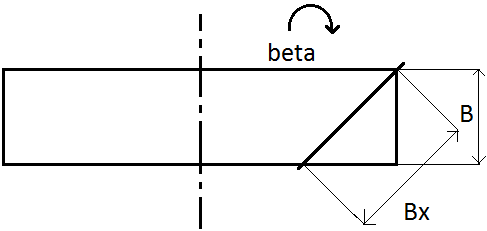
\includegraphics[scale=0.38]{./fig/4.png}
% \caption{\label{fig:4}4} 
% \end{center}
% \end{figure}

\myfig[scale=.28]{figPME2360-20111130-04}{}

\[T_{l,g}=1400K\]
\[cp_{g} = 11205 J/kgK\]
\[\dot{m}_{g}=10kg/s\]
\[\dot{m}_{agua}=3 kg/s\]
Entra x = 0(T=450K)

Sai x = 1 (T=450K)

\[U = 50 W/m^{2}K\]

Lembrando:

\[
\frac{1}{UA}=\frac{1}{U_{f}A_{f}}=\frac{1}{U_{q}A_{q}}=\frac{1}{(\eta_{0}hA)_{f}}+\frac{R_{i,f}^{''}}{(\eta_{0}A)_{f}}+ R_{p}+\frac{K_{i,q}^{''}}{(\eta _{0}A)_{q}} + \frac{1}{(\eta_{0}hA)_{q}}
\]

\[- NUT = \frac{UA}{c_{min}}\]

$c_{min}$, lado dos gases:
\[c_{min}=c_{p,g} \times \dot{m}_{g} = 1120 \times 10 = 11200 W/K\]

Mudança de fase, $c_{vapor} \rightarrow \infty$, $c_{r} \rightarrow 0$

Area de troca?

\[A = 500 \times \pi \times 0.025 \times L = 39.27 \ L\]
\[q_{max} = c_{min} \times (T_{h,e}-T_{c,e}) = 1200 \times (1400 - 450)\]
\[q_{max}= 10.64 \ MW\]
\[q_{trocador}=\dot{m}_{agua} \times h_{lv}\]
Em que $h_{lv}$ = $2024 \times 10^{3} \ J/kg$

\[\varepsilon = \frac{6.07}{10.64}=0.571\]

Trocador de calor com mudança de fase:

\[NUT = -\ln(1-\varepsilon)\]
\[NUT = -\ln(1-0.845)\]
\[NUT = \frac{UA}{c_{min}} = \frac{50 \times 39.27L}{ 11200 }\]
\[L = 4.82 m\]

\section{}

$[...]$água passa por 32 tubos de 50 mm. O aquecimento da água será feito com gases de combustão (calor específico de 1200 J/kg*K) disponíveis a 700º C. A taxa de escoamento dos gases de combustão é de 6000 kg/hr e escoam em um único passe pelo lado do casco. Uma boa estimativa para o coeficiente global de troca de calor, nessa situação, é de 650 $W/m^{2}K$. Pede-se:
\\

a) a temperatura dos gases de aquecimento na saída;

b) a área da troca de calor;

c) o comprimento de cada passe de tubos, considerando-se que o trocador deve ser menor que 1.2 m; 

d) Por necessidade de operação, muda-se a taxa de gases de combustão para 4000 kg/hr e a temperatura de entrada da água para 33º C. Quais serão as novas temperaturas de saída da água e dos gases de combustão, mantida a estimativa do coeficiente global de troca de calor?\\

\subsection{Resolução}

\paragraph{Observação} Como o enunciado do exercício está incompleto (o início da questão foi cortado quando a cópia foi feita), ficaram faltando os valores de temperatura da água na entrada $T_{c,i}$ e na saída $T_{c,o}$ e da taxa de escoamento da água $dot{m}_{c}$. Por isto, será feita apenas uma resolução analítica do exercício para explicar o método de resolução.\\

Tipo de trocador de calor: casco e tubos com um passo no casco

Método a ser usado: $\epsilon$-NUT

\subsubsection{a}

Devemos estimar um valor médio $\bar{T}_{c}$ para a água, para podermos obter o calor específico da água $c_{p,c}$. No caso, 

\[\bar{T}_{c} = \frac{T_{c,o}+T_{c,i}}{2}\]

Consultar a tabela A6 para verificar qual o $c_{p,c}(\bar{T}_{c})$

Calcular $C_{c}$ (água) e $C_{h}$ (gases de combustão)

\[C_{c} = \dot{m}_{c} \times c_{p,c}\]

\[C_{h} = \dot{m}_{h} \times c_{p,h}\]

Calcular q usando os valores que temos de $T_{c,i}$, $T_{c,o}$ e de $C_{c}$

\[q = C_{c} \times (T_{c,o}-T_{c,i})\]

Mas 

\[q = C_{h} \times (T_{h,i}-T_{h,o})\]

Logo

\[T_{h,o} = T_{h,i} - \frac{q}{C_{h}}\]




\subsubsection{b}

Selecionar $C_{min} = \min(C_{c},C_{h})$ e $C_{max} = \max(C_{c},C_{h})$.

Calcular $q_{max}$ com esses valores.

\[q_{max} = C_{min} \times (T_{h,i} - T_{c,i})\]

\[\epsilon = \frac{q}{q_{max}}\]

\[C_{r} = \frac{C_{min}}{C_{max}}\]

Com os valores de $C_{r}$ e de $\epsilon$, usando o gráfico $\epsilon \times$NUT para um trocador de calor casco e tubos com um passe no casco do livro do Incropera para obter o NUT.\\ \\

Com NUT, fazemos:

\[NUT = \frac{U_{h}A_{h}}{C_{min}}\]

\[A_{h}= \frac{C_{min}NUT}{A_{h}}\]


\subsubsection{c}

\[ A_{h} = \pi \times D \times 32 \times L  \] 

\[L = \frac{A_{h}}{\pi \times D \times 32 }\]

O comprimento deve satisfazer $L < 1.2$ m do enunciado
\subsubsection{d}

Calcular o novo valor da capacidade calorífica dos gases de combustão

\[C_{h}' = m_{h}' \times c_{p,h}\]

Obter o novo valor de $C_{min}$

\[C_{min} = \min(C_{c},C_{h}')\]

E então fazemos:

\[C_{r}' = \frac{C_{min}}{C_{max}}\]

\[NUT = \frac{U_{h}A_{h}}{C_{min}}\]

Com NUT e $C_{r}'$, encontramos \[\epsilon'\] através do gráfico $\epsilon \times$NUT para um trocador de calor casco e tubos com um passe no casco do livro do Incropera.

Calculamos $q_{max} = C_{min} (T_{h,i}-T_{o,i})$

Com isso, calculamos q, fazendo:

\[q = \epsilon \times q_{max}\]


E substituimos q em

\[q = C_{h} \times (T_{h,i} - T_{h,o})\]

e 

\[q = C_{c} \times (T_{c,i} - T_{c,o})\]

para obter $T_{h,o}$ e $T_{c,o}$

% \begin{center}
%  \fbox{\input{latex2d}}
%  \end{center}

\begin{figure}[h]
\begin{center}
%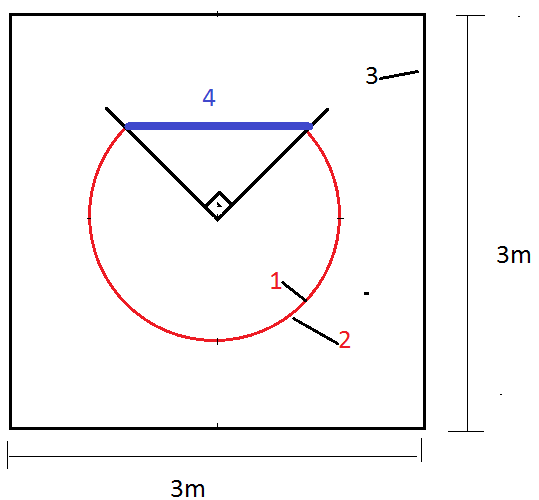
\includegraphics[scale=0.28]{./fig/1.png}
%\caption{\label{fig:1}1} 
\end{center}
\end{figure}

%pme2360
\section{Exercicio 3}
Em um transplante, há necessidade de aquecer e recircular 0.05kg/s do sangue hipotérmico, de 18ºC a 25ºC. Propõe-se fazer isso com um tbo duplo de cobre horizontal, isolado externamente, com diâmetros interno e externo do tubo interior, de 50 e 55mm, e diâmetro interno do tubo exterior, por onde passa a água, de 85mm. O calor específico do sangue é de 3500J/kg.K, e o coeficiente de transferência de calordo lado do sangue é de 100W/$m^2$ºC.

a) Dispondo-se de 0,1kg/s de água a 60ºC, qual é o comprimento do tubo necessário?

b) Ao final da cirurgia deseja-se recuperar a temperatura normal do sangue dos 18ºC para 36ºC. Qual a nova vazão de água necessária?

\textit{Solução}

Calculo da taxa calor trocado:

\[\stackrel{.}{q} = \stackrel{.}{m}_{sangue}\times c_{sangue} \times \Delta T_{sangue}\]

$\stackrel{.}{q} = 0,05 \times 3500 \times (25 - 18) = 1225W$

Calculo da variação de temperatura da água:

Como $\stackrel{.}{m}_{agua}\times c_{agua} >> \stackrel{.}{m}_{sangue}\times c_{sangue}$ e o sangue só varia 7ºC vamos avaliar as propriedades da água para 60ºC.

Tabela A.6:

$c = 4186J/kg.K$

$\mu = 453\times 10^{-6}N.s/m_2$

$k = 656\times 10^{-3}$

\[\stackrel{.}{q} = \stackrel{.}{m}_{agua}\times c_{agua} \times \Delta T_{agua}\]

$1225 = 0,1\times 4186\times ( 60 - T_{agua,2} )$

$T_{agua,2} = 57$ºC

Calculo da temperatura média logaritmica:

\[\Delta T_{ml}= \frac{\Delta T_2 - \Delta T_1}{ln\left(\frac{\Delta T_2}{\Delta T_1}\right)}\]

$\Delta T_{ml}= \frac{(57-18) - (60-25)}{ln\left(\frac{57-18}{60-25}\right)}= 37$ºC

Calculo do coeficiente global de troca de calor:

\[\frac{1}{U_{ext}A_{ext}}=\frac{1}{h_{ext}A_{ext}} + \frac{ln(D_{e}/D_{i})}{2\pi kL} + \frac{1}{h_{int}A_{int}}\]

Para isso é necessário conhecer o $h_{ext}$. Hipótese: Escoamento desenvolvido na região anular e temperatura da superficie não isolada constante.

Usá-se o diâmetro hidráulico $D_{h}= D_{e}-D_{i}$.

\[Re=\frac{4\stackrel{.}{m}_{agua}}{\pi (D_{e}+D{i})\mu}\]

$Re=\frac{4\times 0,1}{\pi \times (85+55)\times 10^{-3}\times 453\times 10^{-6}}= 2008$

Portanto o escoamento é laminar e podemos usar a Tabela 8.2 para determinar Nu.

Fazendo uma interpolação encontramos $Nu_{i}=5,5$ e portanto $h_{ext}=\frac{Nu_{i}k}{D_{h}}=120W/m^2$ºC

Portanto da equação de $U_{ext}$.

$\frac{1}{U_{ext}\pi 55\times 10^{-3}.L}=\frac{1}{120\pi 55\times 10^{-3}.L} + \frac{ln(55/50)}{2\pi 656\times 10^{-3}.L} + \frac{1}{100\pi 50\times 10^{-3}.L}$

$U_{ext}= 43W/m^2$ºC

Finalmente:

\[\stackrel{.}{q} = U_{ext}A_{ext}\Delta T_{ml}\]

$1225=43\times \pi \times 55\times 10^{-3}\times L\times 37$

$L=4,46m$

Para uma variação de 18ºC no sangue:

Calculo do novo $\stackrel{.}{q}$

$\stackrel{.}{q} = 0,05 \times 3500 \times (36 - 18) = 3150W$

Calculo da nova vazão, considerando a mesma variação de temperatura da água.

\[\stackrel{.}{q} = \stackrel{.}{m}_{agua}\times c_{agua} \times \Delta T_{agua}\]

$3150 = \stackrel{.}{m}_{agua}\times 4186 \times 3$

$\stackrel{.}{m}_{agua}= 0,25kg/s$

\include{aulas/pme2360-20111203-ex06}

\include{aulas/pme2360-20111203-ex10}

\end{document}